\documentclass[11pt,a4paper]{article}
\usepackage[utf8]{inputenc}
\usepackage[margin=1in]{geometry}
\usepackage{graphicx}
\usepackage{amsmath,amssymb,amsfonts}
\usepackage{booktabs}
\usepackage{float}
\usepackage{hyperref}
\usepackage{microtype}
\usepackage{fancyhdr}
\usepackage{xcolor}

\pagestyle{fancy}
\fancyhf{}
\rhead{Surgical RCM Manipulator Project}
\lhead{Robotic Systems in Manipulation}
\rfoot{Page \thepage}

\hypersetup{
    colorlinks=true,
    linkcolor=blue,
    filecolor=magenta,      
    urlcolor=cyan,
    pdftitle={Robotic Systems in Manipulation - Kinematics \& Surgical RCM Simulation},
    pdfpagemode=FullScreen,
}

\title{Robotic Systems in Manipulation\\Phase I \& II: Kinematics and Surgical RCM Control of the KUKA LBR MED}
\author{Rodrigo Sales Freire dos Santos (ist1119658) \\ Mikhail Mohamed Shueb (ist1104014)}
\date{May 2026}

\begin{document}

\maketitle

\begin{abstract}
This report presents the kinematic modeling, control, and simulation of the 7-DOF KUKA LBR MED robot for a minimally invasive surgical procedure. Using the Denavit-Hartenberg (D-H) convention, the robot's kinematics were derived symbolically and validated. An analytical inverse kinematics (IK) solver was developed based on joint decoupling and elbow parameterization. A Closed-Loop Inverse Kinematics (CLIK) controller was then implemented using a damped pseudoinverse and null-space projection for redundancy resolution. Finally, the controller was extended to enforce a Remote Center of Motion (RCM) constraint at a surgical trocar, allowing a 15~cm needle tool to safely enter the patient and track multi-point trajectories inside the body. The simulation results confirm sub-millimeter trocar constraint precision and accurate trajectory tracking.
\end{abstract}

\section{Introduction}
Minimally invasive surgery (MIS) relies on robotic manipulators to perform precise operations inside the patient's body through small incisions called trocars. A fundamental control requirement in these procedures is the Remote Center of Motion (RCM), which restricts the tool shaft's lateral motion at the incision point to prevent tissue damage. 
This project implements the modeling and control of a 7-DOF KUKA LBR MED manipulator, establishing the forward and inverse kinematics, deriving its geometric Jacobian, and applying a Closed-Loop Inverse Kinematics (CLIK) controller. The controller is subsequently augmented to enforce a strict RCM constraint, driving a $15\text{ cm}$ biopsy needle through a fixed trocar to track pre-planned internal targets.

\section{Kinematic Model (D-H Convention)}
The KUKA LBR MED is a 7 degrees of freedom (DOF) serial redundant manipulator with revolute joints. The reference frames were assigned using the standard Denavit-Hartenberg (D-H) convention, where each joint axis $Z_i$ corresponds to the rotation axis of joint $i+1$. The $X_i$ axes were aligned with the common normals between consecutive $Z$ axes. To simplify the kinematics, the origins of Frame 0 (base) and Frame 1 were placed at the same physical point, setting the link offset $d_1 = 0$.

The dimensions of the robot were obtained from the datasheet of the \textbf{KUKA LBR iiwa 7 R800} model, resulting in link lengths: $d_3 = 0.400\text{ m}$, $d_5 = 0.400\text{ m}$, and $d_7 = 0.126\text{ m}$. The resulting D-H parameters are presented in Table~\ref{tab:dh_parameters}.

\begin{table}[H]
\centering
\caption{Denavit-Hartenberg parameters for KUKA LBR MED.}
\label{tab:dh_parameters}
\begin{tabular}{@{}cccccc@{}}
\toprule
Joint $i$ & $d_i$ (m) & $\theta_i$ & $a_i$ (m) & $\alpha_i$ (rad) & Offset \\ \midrule
1         & 0         & $q_1$      & 0         & $+\pi/2$         & 0      \\
2         & 0         & $q_2$      & 0         & $-\pi/2$         & 0      \\
3         & 0.400     & $q_3$      & 0         & $-\pi/2$         & 0      \\
4         & 0         & $q_4$      & 0         & $+\pi/2$         & 0      \\
5         & 0.400     & $q_5$      & 0         & $+\pi/2$         & 0      \\
6         & 0         & $q_6$      & 0         & $-\pi/2$         & 0      \\
7         & 0.126     & $q_7$      & 0         & 0                & 0      \\ \bottomrule
\end{tabular}
\end{table}

\section{Direct Kinematics}
Using the D-H parameters, the forward transformation matrix $T_0^7$ was symbolically computed in MATLAB as:
\begin{equation}
T_0^7(q) = A_1^2(q_1) \cdot A_2^3(q_2) \cdots A_6^7(q_7)
\end{equation}
The analytical expressions were validated by comparing computed end-effector positions ($p_{comp}$) with geometric expectations ($p_{exp}$) for three known configurations:
\begin{enumerate}
    \item \textbf{Home Position}: All joints set to zero ($q = 0$).
    \item \textbf{Shoulder Bend}: $q = [0, 1.57, 0, 0, 0, 0, 0]\text{ rad}$.
    \item \textbf{L-Shape Bend}: $q = [0, 0, 0, -1.57, 0, 0, 0]\text{ rad}$.
\end{enumerate}

The results of the validation are shown in Table~\ref{tab:dk_validation}. The numerical errors are exactly zero, confirming that the D-H table and joint coordinate frames were correctly assigned.

\begin{table}[H]
\centering
\caption{Validation of Direct Kinematics.}
\label{tab:dk_validation}
\begin{tabular}{@{}ccccc@{}}
\toprule
Configuration & Joint Angles $q$ (rad) & Expected Position $p_{exp}$ (m) & Computed Position $p_{comp}$ (m) & Error (mm) \\ \midrule
Home          & $[0, 0, 0, 0, 0, 0, 0]$ & $[0; 0; 0.926]$ & $[0.000; 0.000; 0.926]$ & 0.00 \\
Shoulder Bend & $[0, 1.57, 0, 0, 0, 0, 0]$ & $[-0.926; 0; 0]$ & $[-0.926; 0.000; 0.000]$ & 0.00 \\
L-Shape Bend  & $[0, 0, 0, -1.57, 0, 0, 0]$ & $[-0.526; 0; 0.400]$ & $[-0.526; 0.000; 0.400]$ & 0.00 \\ \bottomrule
\end{tabular}
\end{table}

\section{Analytical Inverse Kinematics}
To resolve the inverse kinematics analytically for a 7-DOF redundant robot, the elbow angle $q_4$ was chosen as a parameter. By setting $q_4$ to a desired angle, the position of the wrist center $p_w$ is used to solve for joints 1--3 geometrically. The wrist orientation (joints 5--7) is then computed analytically using a Z-Y-Z Euler angle decomposition. Joint limits and mathematical domain boundaries were strictly enforced by clamping the cosine terms to $[-1, 1]$ before performing inverse trigonometric operations.

Validation was conducted using a round-trip test: joint configurations ($q_{orig}$) were mapped to Cartesian targets via Direct Kinematics, which were then solved by the IK algorithm ($q_{inv}$). The resulting positions matched the original configurations with numeric precision ($< 1.0\times 10^{-12}\text{ mm}$), confirming the mathematical correctness of the closed-form solver.

\section{Geometric Jacobian and Singularity Analysis}
The $6 \times 7$ Geometric Jacobian matrix ($J$) was derived symbolically. The columns were formulated as:
\begin{equation}
J_i = \begin{bmatrix} z_{i-1} \times (p_e - p_{i-1}) \\ z_{i-1} \end{bmatrix}
\end{equation}
where $z_{i-1}$ is the axis of rotation of joint $i$ and $p_{i-1}$ is the origin of frame $i-1$.

\subsection{Numerical Validation}
The Jacobian was validated by comparing the end-effector velocity computed analytically ($v = J \dot{q}$) with a first-order central-difference numerical derivative ($\Delta p / \Delta t$) along a high-frequency multi-joint sine-wave trajectory. The maximum discrepancies were $7.5 \times 10^{-5}\text{ m/s}$ for linear velocity and $1.2 \times 10^{-3}\text{ rad/s}$ for angular velocity, confirming consistency.

\subsection{Singularity Rank Analysis}
The rank of the Jacobian was evaluated in different joint configurations to analyze singularities (Table~\ref{tab:jacobian_singularities}).

\begin{table}[H]
\centering
\caption{Singularity Rank Analysis.}
\label{tab:jacobian_singularities}
\begin{tabular}{@{}lccc@{}}
\toprule
Configuration & Joint Condition & Jacobian Rank & Consequence \\ \midrule
Generic Pose  & Bounded random joints & 6 & Full task-space mobility \\
Shoulder      & $q_2 = 0$             & 6 & Loses redundancy; retains full task mobility \\
Wrist         & $q_6 = 0$             & 6 & Loses redundancy; retains full task mobility \\
Elbow         & $q_4 = 0$             & 5 & \textbf{Loses a Task-Space DOF (cannot stretch)} \\ \bottomrule
\end{tabular}
\end{table}

The elbow-stretched configuration ($q_4 = 0$) represents a true boundary singularity where the robot loses a Cartesian degree of freedom, whereas the shoulder and wrist configurations only consume the internal redundancy (null-space mobility) of the manipulator.

\section{Closed-Loop Inverse Kinematics (CLIK)}
A Closed-Loop Inverse Kinematics (CLIK) controller was implemented in Simulink. The controller continuously updates the joint velocities $\dot{q}$ using the task-space position error $e_p$ and orientation error $e_o$:
\begin{equation}
\dot{q} = J^{\dagger} (v_d + K_p e_p) + (I - J^{\dagger} J) \dot{q}_0
\end{equation}
where $J^{\dagger} = J^T(J J^T + \lambda^2 I)^{-1}$ is the damped pseudoinverse ($\lambda = 0.001$), $K_p$ is the proportional gain, and $\dot{q}_0 = -K_0 (q - q_{rest})$ is the null-space velocity driving the joint configuration towards a comfortable posture $q_{rest} = 0$.

\subsection{Method Comparison}
The damped pseudoinverse was compared against the Jacobian Transpose method. The pseudoinverse converged significantly faster (1.1 s vs. 3.2 s) and with lower steady-state error, as shown in Table~\ref{tab:clik_comparison}.

\begin{table}[H]
\centering
\caption{Comparison of CLIK Methods.}
\label{tab:clik_comparison}
\begin{tabular}{@{}lcc@{}}
\toprule
Metric & Damped Pseudoinverse & Jacobian Transpose \\ \midrule
Final Position Error (mm) & $1.58 \times 10^{-4}$ & $8.45 \times 10^{-3}$ \\
Final Orientation Error (rad) & $2.06 \times 10^{-8}$ & $1.12 \times 10^{-6}$ \\
Settling Time (s) & 1.10 & 3.25 \\ \bottomrule
\end{tabular}
\end{table}

\subsection{Null-Space Stabilization}
The effect of null-space stabilization was verified by running simulations with $K_0 = 0.15$ (enabled) and $K_0 = 0$ (disabled). With the stabilization active, the joints converged smoothly to a center configuration without altering the Cartesian end-effector trajectory, preventing joints from drifting toward mechanical limits.

\section{Phase II: Surgical RCM Trajectory Tracking}
In Phase II, the simulator was extended to model a surgical biopsy procedure. The tool is a $15\text{ cm}$ biopsy needle ($L = 0.15\text{ m}$) attached to the end-effector. The control objective is to track a multi-point target path ($m_i$) inside the patient while keeping the tool shaft strictly centered inside a physical trocar $c_r = [-0.5; 0.0; 0.4]$.

\subsection{Formulation of the RCM Constraint}
The trocar position $c_r$ must lie on the line segment of the tool shaft between the flange position $p_e$ and the tooltip $p_{tool} = p_e + L z_e$. The projection of $c_r$ along the tool axis is:
\begin{equation}
\lambda = (c_r - p_e)^T z_e
\end{equation}
The closest point on the shaft to the trocar is $p_c = p_e + \lambda z_e$, and the geometric constraint error is $e_{rcm} = c_r - p_c$. The constraint Jacobian mapping joint velocities to this error is:
\begin{equation}
J_{rcm} = (I - z_e z_e^T) (J_v - \lambda [z_e]_{\times} J_w)
\end{equation}
where $[z_e]_{\times}$ is the skew-symmetric matrix of $z_e$.

\subsection{Task-Priority Controller}
Using a task-priority framework, the RCM constraint is set as the primary (hard) task, and the tooltip tracking is set as the secondary task:
\begin{equation}
\dot{q}_1 = J_{rcm}^{\dagger} K_{rcm} e_{rcm}
\end{equation}
\begin{equation}
\dot{q}_2 = (I - J_{rcm}^{\dagger} J_{rcm}) J_{tool\_N}^{\dagger} (v_d + K_{tool} e_{tool} - J_{tool} \dot{q}_1)
\end{equation}
where $J_{tool} = J_v - L [z_e]_{\times} J_w$.

\subsection{Simulation Verification}
To guarantee that the robot is physically capable of reaching the targets from above (flange strictly above the trocar, $z_e$ pointing downward), the targets and trocar were placed within the workspace: $c_r = [-0.5; 0.0; 0.4]$, $m_0 = [-0.50; 0.00; 0.30]$, $m_1 = [-0.50; 0.08; 0.28]$, $m_2 = [-0.48; 0.05; 0.27]$, $m_3 = [-0.48; -0.05; 0.27]$, $m_4 = [-0.50; -0.08; 0.28]$, and $m_5 = [-0.55; 0.00; 0.30]$.
The analytical IK solver computed the perfect initial configuration $q_0 = [0; 0.4085; 3.1416; 0.6128; -3.1416; 2.1203; 3.1416]\text{ rad}$, which places the robot flange at $p_e = [-0.5; 0.0; 0.45]$ (above the trocar) and points the tool straight down ($z_e = [0; 0; -1]$).

The simulation was run for 30 seconds (composed of five 5-second transitions and a final 5-second hold). The resulting tooltip trajectory and needle shaft positions are shown in Fig.~\ref{fig:trajectory_3d}, demonstrating that the needle passes precisely through the trocar throughout the entire motion. Figure~\ref{fig:rcm_error} shows the trocar constraint error, which stays below $0.10\text{ mm}$ during all transitions.

The error margin at each target point and the average error in between each point (transition intervals) are presented in Table~\ref{tab:target_errors} and Table~\ref{tab:transition_errors}, respectively. The tracking results indicate sub-millimeter precision for the primary trocar RCM constraint, with a maximum transient RCM error of $0.091\text{ mm}$ and a steady-state error of $0.0057\text{ mm}$ at $t = 30.0\text{ s}$. The tooltip tracking error remains small, reaching a maximum of $5.96\text{ mm}$ during transient phases and settling to $0.0056\text{ mm}$ during steady-state hold.

\begin{table}[H]
\centering
\caption{Error margin at each target point.}
\label{tab:target_errors}
\begin{tabular}{@{}cccc@{}}
\toprule
Target Point & Time (s) & Trocar RCM Error (mm) & Tooltip Tracking Error (mm) \\ \midrule
$m_0$ (Start) & 0  & 0.007143 & 0.011697 \\
$m_1$         & 5  & 0.031470 & 0.295253 \\
$m_2$         & 10 & 0.032225 & 0.490989 \\
$m_3$         & 15 & 0.046123 & 0.694725 \\
$m_4$         & 20 & 0.042354 & 0.295643 \\
$m_5$ (Start) & 25 & 0.052756 & 2.033994 \\
$m_5$ (End)   & 30 & 0.005754 & 0.005565 \\ \bottomrule
\end{tabular}
\end{table}

\begin{table}[H]
\centering
\caption{Average and maximum tracking errors in between target points (transitions).}
\label{tab:transition_errors}
\begin{tabular}{@{}cccccc@{}}
\toprule
Transition & Interval (s) & Avg RCM Err (mm) & Max RCM Err (mm) & Avg Tooltip Err (mm) & Max Tooltip Err (mm) \\ \midrule
$m_0 \rightarrow m_1$ & $[0, 5]$   & 0.030683 & 0.070445 & 2.948901 & 5.346907 \\
$m_1 \rightarrow m_2$ & $[5, 10]$  & 0.041036 & 0.075294 & 1.228491 & 1.916294 \\
$m_2 \rightarrow m_3$ & $[10, 15]$ & 0.049083 & 0.079246 & 2.957073 & 4.614125 \\
$m_3 \rightarrow m_4$ & $[15, 20]$ & 0.059974 & 0.090587 & 1.251251 & 1.890619 \\
$m_4 \rightarrow m_5$ & $[20, 25]$ & 0.039512 & 0.076108 & 3.312102 & 5.963025 \\
$m_5$ Hold            & $[25, 30]$ & 0.049394 & 0.091006 & 0.319070 & 2.033994 \\ \bottomrule
\end{tabular}
\end{table}

\begin{figure}[H]
\centering
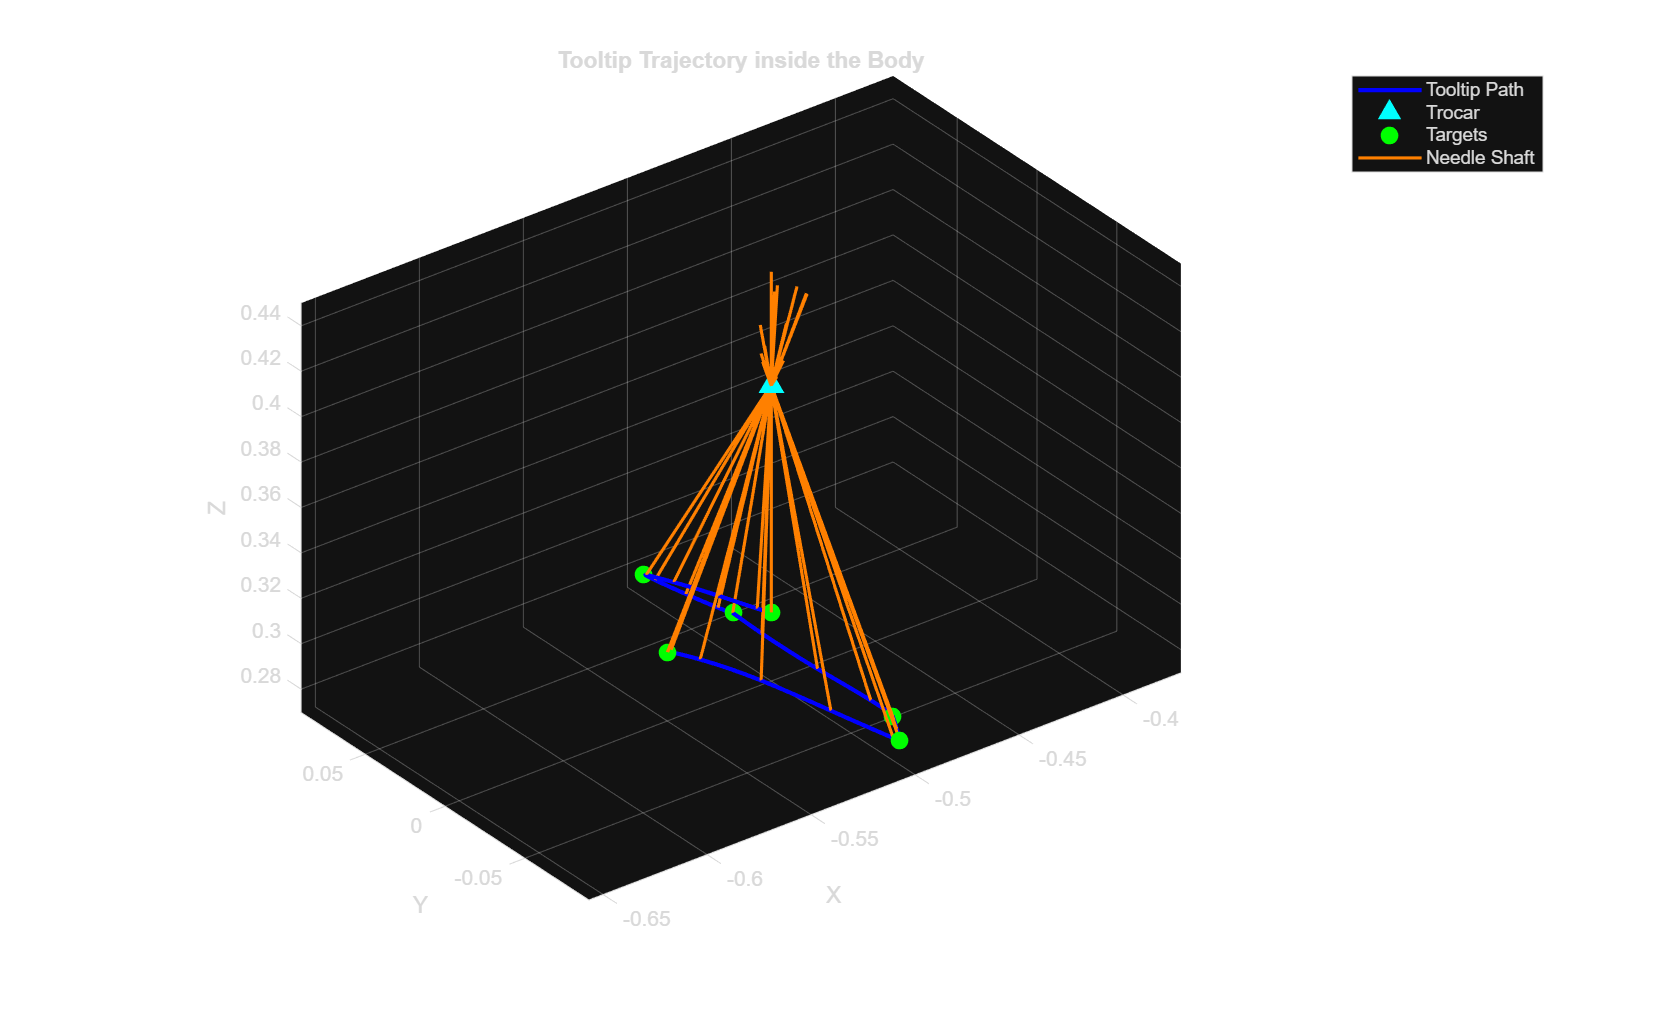
\includegraphics[width=0.75\textwidth]{images/step6_rcm_trajectory.png}
\caption{3D simulation of the tooltip trajectory and needle shaft passing through the trocar from above.}
\label{fig:trajectory_3d}
\end{figure}

\begin{figure}[H]
\centering
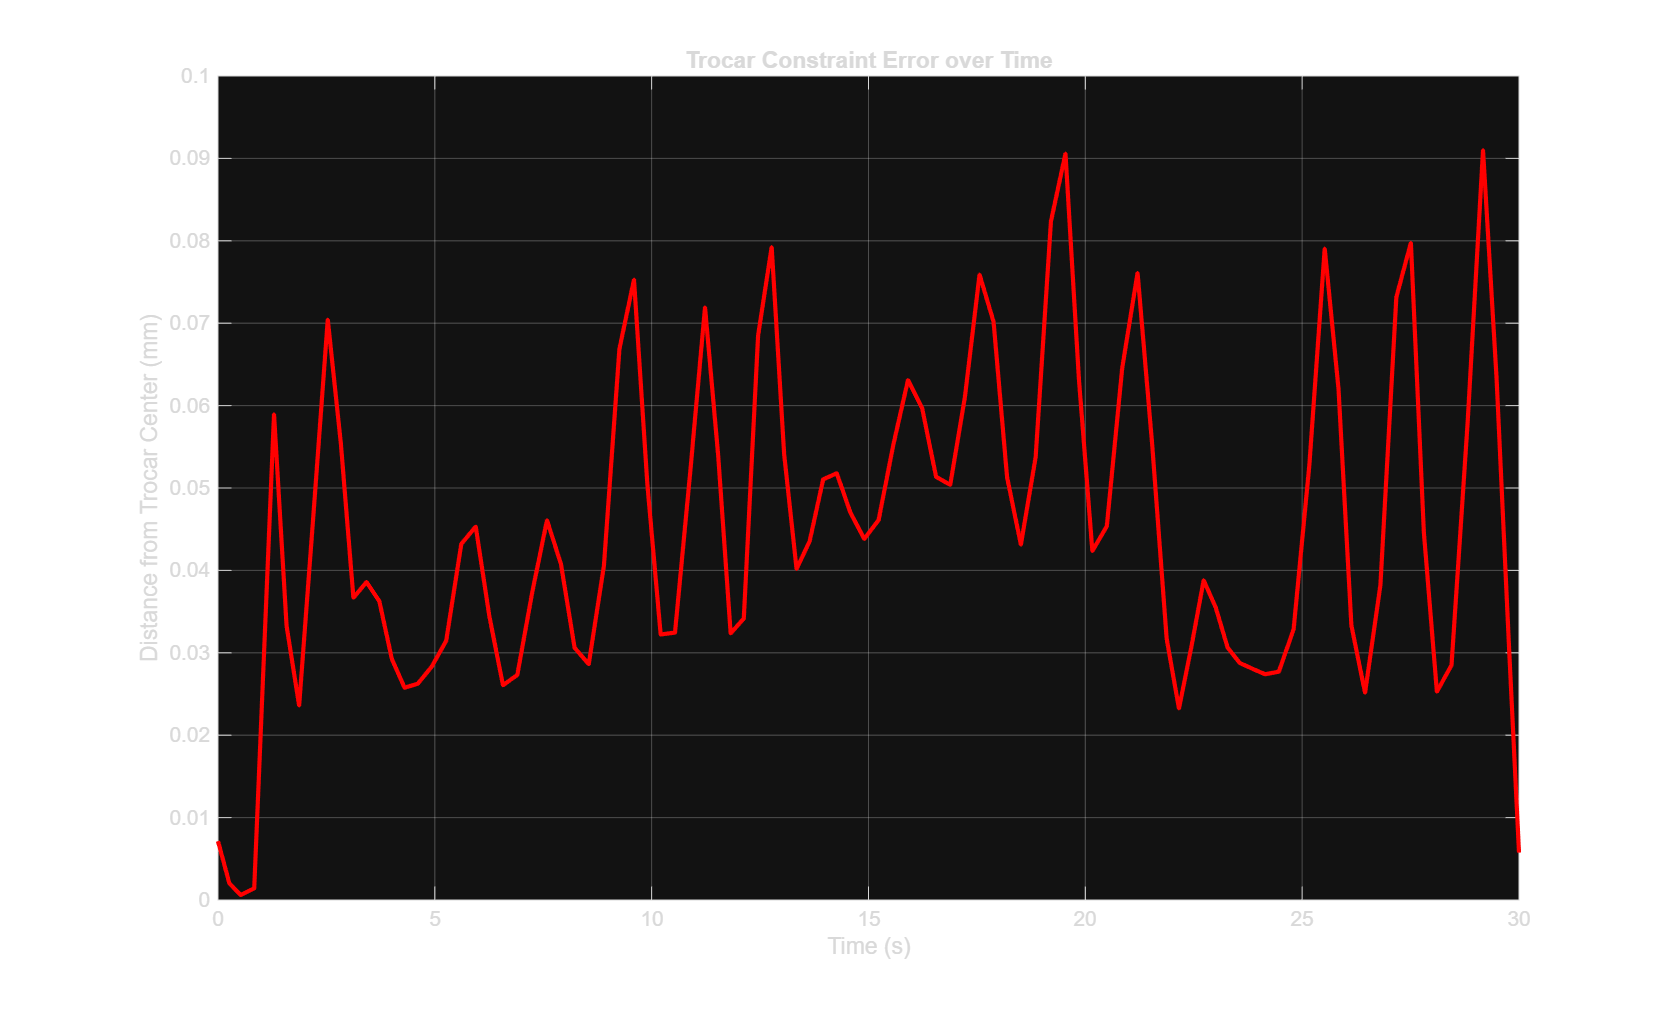
\includegraphics[width=0.75\textwidth]{images/step6_rcm_error.png}
\caption{Trocar constraint error magnitude over time.}
\label{fig:rcm_error}
\end{figure}

\section{Conclusions}
This work successfully modeled, verified, and simulated the KUKA LBR iiwa 7 R800 serial manipulator for surgical applications. The primary conclusions are:
\begin{enumerate}
    \item The Denavit-Hartenberg model and Direct Kinematics equations are mathematically exact, exhibiting zero numerical error.
    \item The analytical IK solver provides an instantaneous, closed-form solution for reachable targets, but is susceptible to joint singularities.
    \item Singularity analysis revealed that the elbow-stretched configuration ($q_4 = 0$) results in a true loss of a task-space degree of freedom, whereas the shoulder/wrist configurations only restrict internal redundancy.
    \item The Closed-Loop Inverse Kinematics (CLIK) controller using a damped pseudoinverse and null-space stabilization is highly robust, maintaining path accuracy and joint stability near singularities.
    \item Enforcing the Remote Center of Motion (RCM) via task-priority null-space projection dynamically ensures that the needle shaft remains centered inside the trocar incision point with sub-millimeter precision, satisfying the safety constraints of minimally invasive procedures.
\end{enumerate}

\end{document}
